\section{Evaluation}
	\begin{itemize}
	\squish
		\item Ranking of organization according to the impact w.r.t to approved patents
		\item Plot of invention impact vs collaborative distance to answer Question 1
		\item Plot of invention impact vs organization to answer Question 2
		\item Plot of collaborative distance vs organization to answer Question 3
	\end{itemize}

\begin{table*}[t] 
  %\centering
  \begin{tabular}{@{}c@{}} 
  \begin{minipage}{0.4\linewidth}
		\begin{center}
	  		\begin{tabular}{| l | l |}
				\hline
				{Type} & {Count} \\
				\hline
				\hline
				Inventors (Nodes) & 0.96 \\
				Co-authorships (Edges) & 1.29 \\
				Patents & 123123 \\
				Source Node & Thomas Edison\\
				Avg. Distance & 1.33 \\
				\hline
			\end{tabular}		
			\caption {Should be a caption}

			\vspace{0.85cm}

			\begin{tabular}{| l | l |}
				\hline
				{Algorithm} & {Time} \\
				\hline
				\hline
				Algo I & 0.96 \\
				Algo II & 1.29 \\
				Algo III & 1.33 \\
				\hline
			\end{tabular}
			\caption {Should be a caption}
		\end{center}

  \end{minipage}
  \hspace{0.05\linewidth}
  \begin{minipage}{0.45\linewidth}
      \begin{figure}[H]
          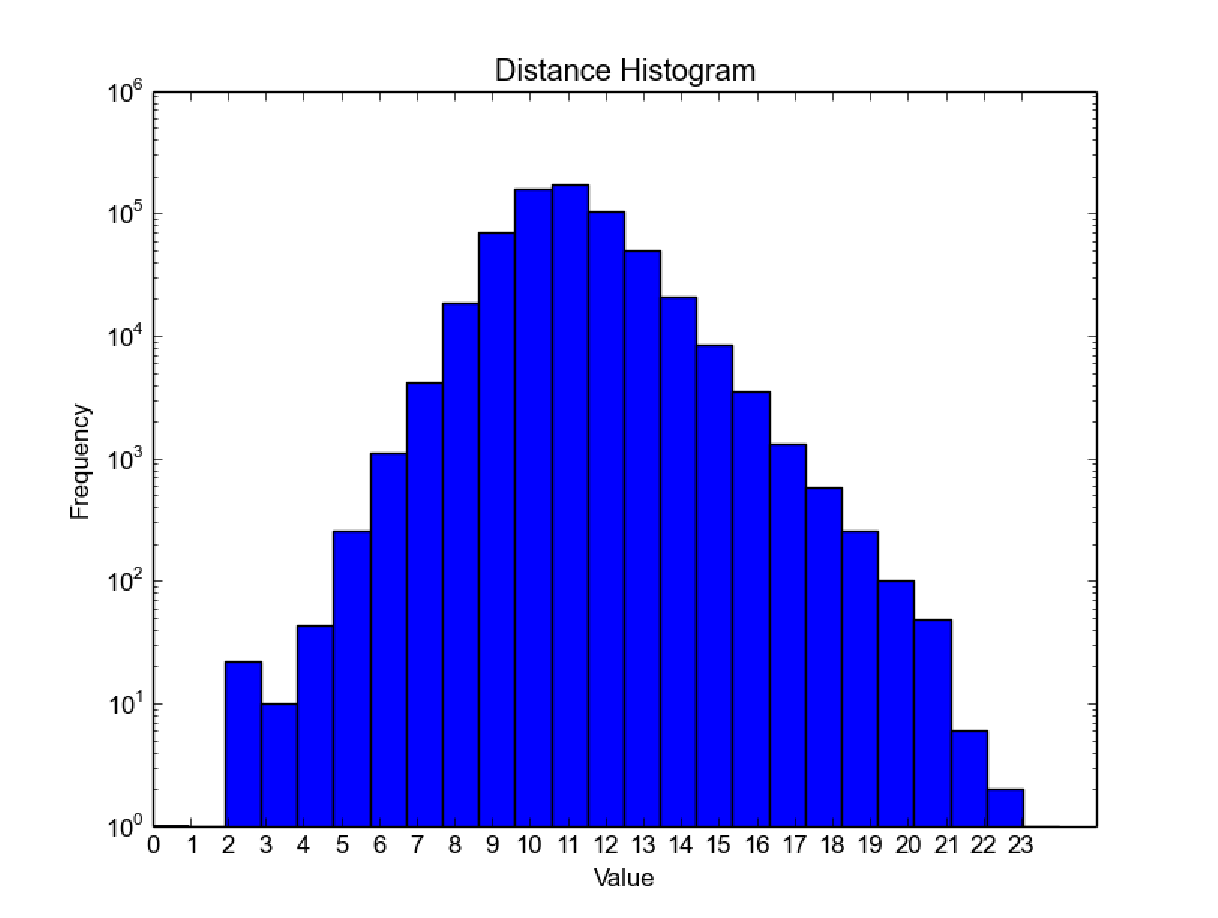
\includegraphics[scale=0.425]{../figures/distance.pdf}
          \caption{This is the second figure}
      \end{figure}
  \end{minipage}
  \end{tabular}
\end{table*}

% \end{minipage}

\begin{table*}[t] 
  %\centering
  \begin{tabular}{@{}c@{}} 
   \begin{minipage}{0.45\linewidth}
      \begin{figure}[H]
          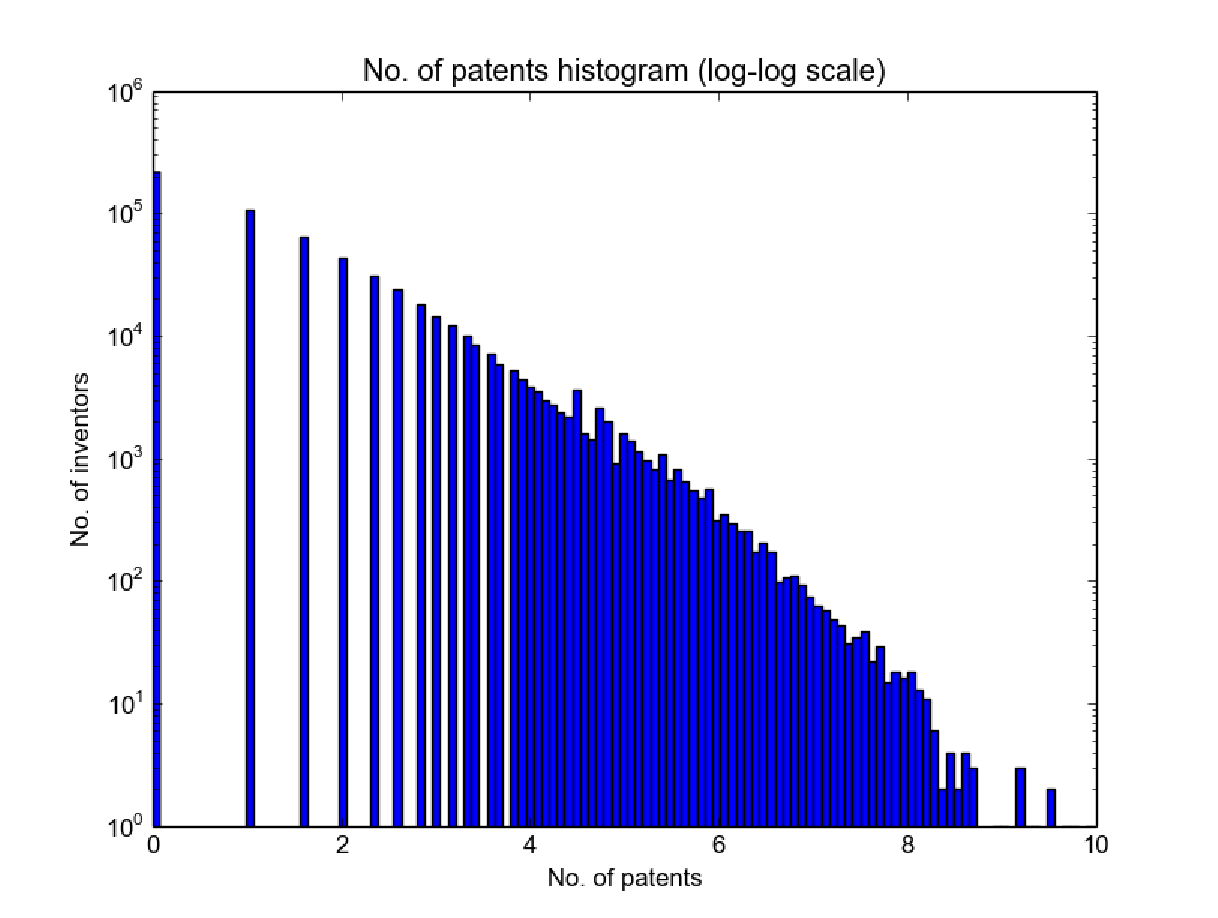
\includegraphics[scale=0.425]{../figures/patent.pdf}
          \caption{This is the third figure}
      \end{figure}
  \end{minipage}
  \begin{minipage}{0.45\linewidth}
      \begin{figure}[H]
          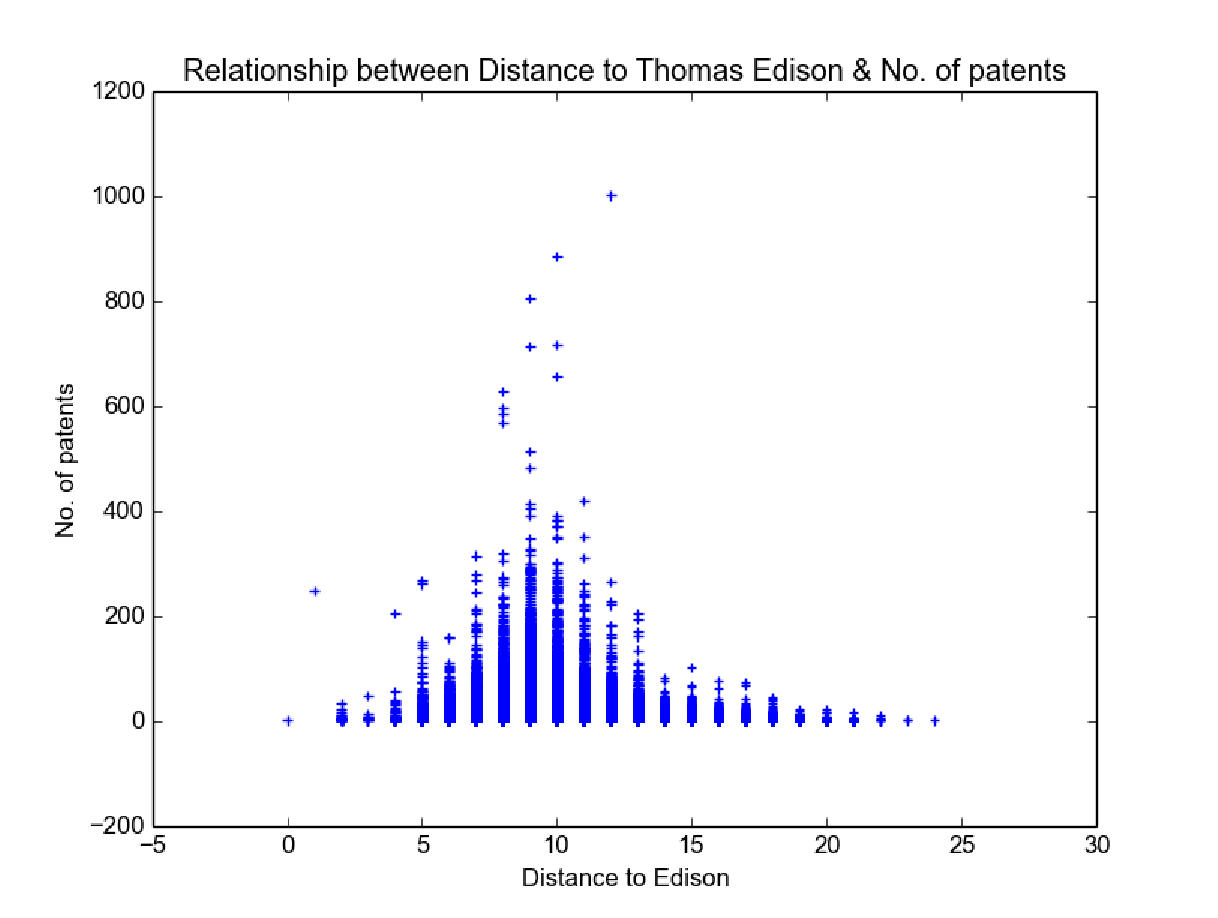
\includegraphics[scale=0.425]{../figures/distance_patent.pdf}
          \caption{This is the first figure}
      \end{figure}
  \end{minipage}
  \end{tabular}
\end{table*}
